\documentclass[a4paper,12pt]{article}
\usepackage{graphicx} % Ensures graphicx is loaded
\usepackage{geometry} % Page margins
\usepackage{amsmath} % For math formatting
\geometry{left=2.5cm,right=2.5cm,top=2.5cm,bottom=2.5cm}
\usepackage{fancyhdr} % Header and footer
\usepackage{titlesec} % Section format
\usepackage{listings} % Code environment
\usepackage{xcolor} % Colors
\usepackage{hyperref} % Hyperlinks
\usepackage{array} % For table formatting

\usepackage{url}

% Define the custom color for background
\definecolor{mycolor}{RGB}{255, 255, 255}

\begin{document}

\pagecolor{mycolor}

% Custom title layout
% Custom title layout
\begin{titlepage}
    \begin{center}
        % Title
        {\Huge \textcolor{black}{\textbf{User Manual}}}
        \vspace{1.5cm} % Adjust spacing below the title as needed
        
        % Logo at the top
        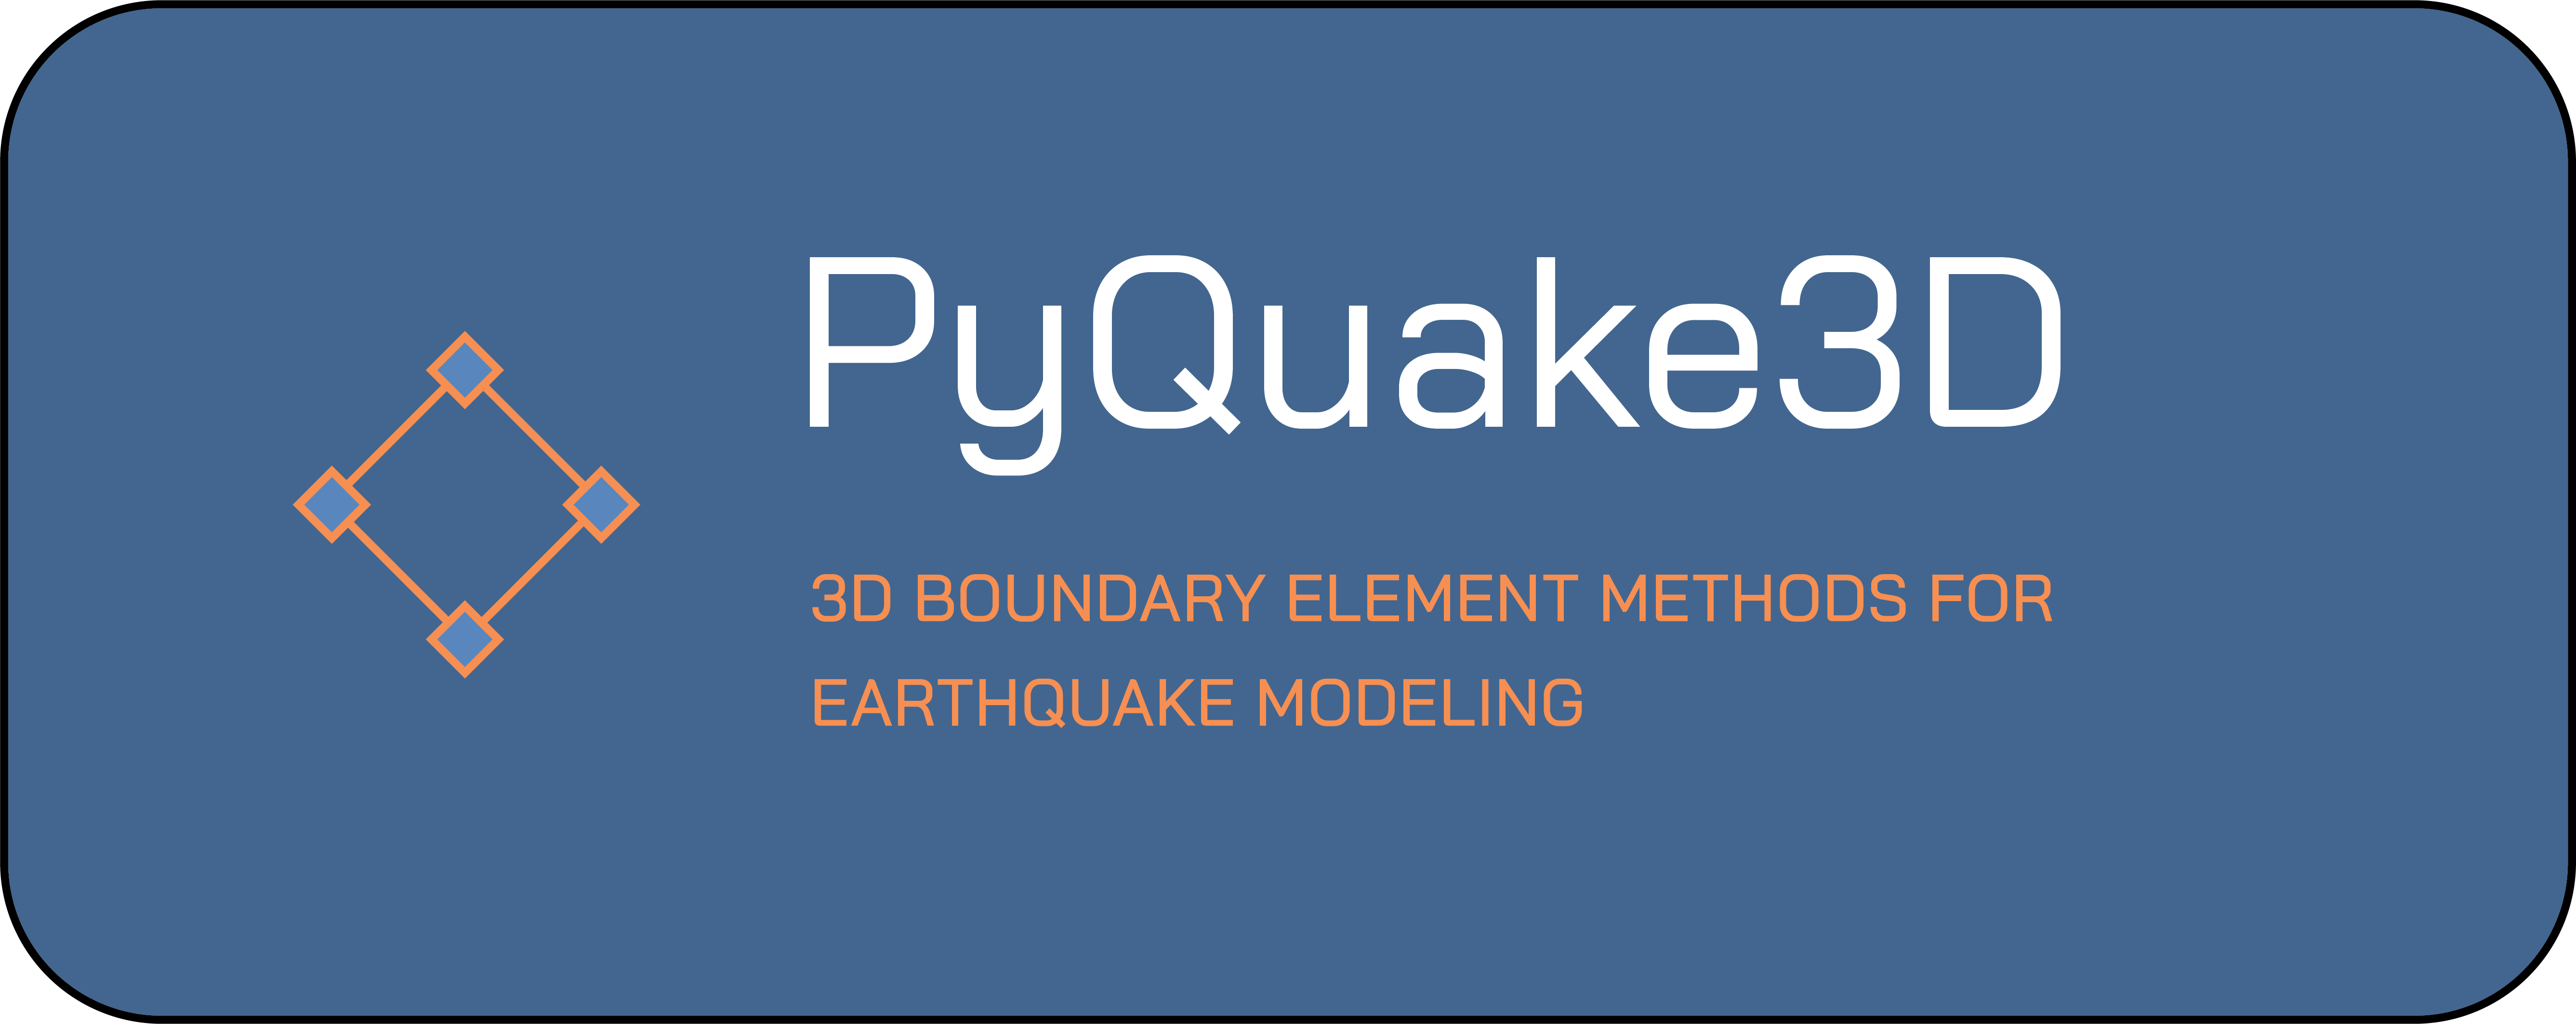
\includegraphics[width=1.0\textwidth]{Logo-PyQuake3D.png}
        \vspace{1.5cm} % Adjust spacing below the logo as needed

        % Author information
        {\large \textcolor{black}{Rongjiang TANG\footnotemark[1] \& Luca DAL ZILIO\footnotemark[2]}}
        \vspace{1.5cm} % Adjust spacing below the author information as needed
        
        % Date
        \vspace{1cm} % Adjust spacing below the author information
        {\large \textcolor{black}{\today}}
        
    \end{center}

    % Define footnotes for emails
    \footnotetext[1]{\textcolor{black}{\url{rongjiang.igp@hotmail.com}}}
    \footnotetext[2]{\textcolor{black}{\url{luca.dalzilio@ntu.edu.sg}}}

\end{titlepage}

\pagecolor{white}

% Table of Contents
\newpage
\tableofcontents
\newpage

% Introduction
\section{Introduction}
PyQuake3D is a \textbf{Python}-based Boundary Element Method (BEM) code for simulating sequences of seismic and aseismic slip (SEAS) on a complex 3D fault geometry governed by rate- and state-dependent friction. It can handle arbitrary 3D fault geometries in either uniform elastic half-space or full-space scenarios, including simulations of non-planar, branches, step-over, and rough faults. This document provides an overview of how to use the script, as well as a detailed description of the input parameters.

\section{Contribution}
2024.7.1  Rongjiang Tang developed the code framework and the Quasi-dynamic BIEM Seismic cycle model on a complex 3D fault geometry governed by regularized aging law.\\

2024.10.5 Rongjiang Tang and Luca Dal Zilio implemented the H-matrix Matrix-Vector Multiplication and developed the Cascadia model.

We welcome contributions to PyQuake3D. Please ensure that you follow the contribution guidelines and maintain the consistency of the codebase.

\section{Dependencies}

\begin{align*}
    \text{Python} &\geq 3.8 \\
    \text{NumPy} &\geq 1.2 \\
    \text{ctypes} &== 1.1
\end{align*}


Generally, the numpy library comes pre-installed with Python. The ctypes is a library used for calling C code from Python, and it can be installed using:

$pip$ $install$ $ctypes$

\section{How to run}
Download the source codes from github. Type:

To run the PyQuake3D script, use the following command\\
\texttt{python -g --inputgeo <input\_geometry\_file> -p --inputpara <input\_parameter\_file>}\\

For example,To execute benchmarks like BP5-QD at Current Directory\\
\texttt{python src/main.py -g --examples/bp5t/bp5t.msh -p --examples/bp5t/parameter.txt}\\

To run cascadia model, use:\\
\texttt{python src/main.py -g --examples/cascadia/cascadia35km\_ele4.msh -p \\--examples/cascadia/parameter.txt}\\

Ensure that the `parameter.txt` file in each example is appropriately configured as described in the parameter setting description.

\section{Code Structure and file description}
All the python codes are located in the $src$ directory, and parameters and models can be found in the examples folder. H2lib is a C language H-matrix library used to compile the dynamic library hm.so, which allows Python to call the H2lib C programs to use H-Matrix. Generally, you do not need to recompile the library, as we have already compiled the dynamic library in a Linux environment and placed it in the src directory. However, if you are using macOS or need to modify the C code, you will need to recompile and link the code in the $H2lib-master$ directory using make, and then replace the original hm.so file in the $src$ directory with the newly compiled version.

The examples directory contains three subdirectories, each with an example. The $bp5t$ directory contains the benchmark half-space fault model published by the Southern California Earthquake Center (https://strike.scec.org/cvws/seas/download/ ). The $Cascadia$ directory simulates the Cascadia subduction zone, based on the publicly available slab2 model (https://www.sciencebase.gov/catalog/item/5aa1b00ee4b0b1c392e86467). Surface0 is a simple half-space non-planar fault surface model used for testing simulation results for non-planar condition. The $bp5t$ and $Cascadia$ requires external input for initial conditions, while $surface0$ allows initial conditions to be set through $parameter.txt$.



The code consists of multiple modules as the following functions:
\begin{itemize}
    \item \textbf{main.py}: Executing the quasi-dynamic model program, allow the user to code for output
    \item \textbf{QDsim.py}: Class for establishing a quasi-dynamic model
    \item \textbf{DH\_Greenfunction.py}: Calculate stress green functions in homogeneous Elastic Half-Space
\item \textbf{SH\_Greenfunction.py}: Calculate stress green functions in homogeneous Elastic Full-Space.
\item \textbf{Readmsh.py}: Reading External Data and parameters
\item \textbf{Hmatrix.py}: Load dynamic library
\end{itemize}

% Table for Module Parameters
\section{Parameters setting}
The simulation parameters are implemented by modifying the $parameter.txt$ file, rather than by changing the source code. The input variable list is in $Table$ \ref{tab:module_params}. If $InputHetoparamter$ in $Table$ \ref{tab:module_params} is True, heterogeneous stress and friction parameters are imported from external files. The external filename is defined in $parameter.txt$ and must remain in the same directory as $parameter.txt$. In this case, you only need to appropriately set parameter of $Table$ \ref{tab:module_params} and $Table$ \ref{tab:Output Setting}. Otherwise, you need to appropriately set the parameters of stress and frictional initial condition shown in  $Table$ \ref{tab:Stress and Frition  Settings} and $Table$ \ref{tab:Nucleation and Friction Setting}.



\begin{table}[h!]
    \centering
    \caption{General Parameters}
    \label{tab:module_params}
    \begin{tabular}{|m{3.5cm}|m{2cm}|m{9cm}|}
        \hline
        \textbf{Parameter} & \textbf{Default} & \textbf{Description} \\
        \hline
        \texttt{Corefunc directory} &  & The storage path for the kernel function matrix composed of stress Green's functions \\
        \hline
        \texttt{Input Hetoparamter} &  False & If `True`, the heterogeneous stress and friction parameters are imported from external files. \\
        \hline
        \texttt{Inputparamter file} &  & The file name of imported heterogeneous stress and friction parameters \\
        \hline
	\texttt{Processors} & 50 & The number of processors which can be scheduled by the operating system to run on different CPU cores. \\
        \hline
	\texttt{Batch\_size} & 1000 & The number of processes which can be scheduled by the operating system to run on different CPU cores. \\
        \hline
	\texttt{H-matrix} & False & If `True`, The kernel function will be approximated using H-Matrix. Note that in this case, the code must be run under Linux or MacOS system. The H-Matrix approximation is implemented using the open-source C library $H2Lib$, and the compilation of the dynamic library is done based on Makefile in $H2Lib-master$ directory. \\
\hline	
\texttt{Lame constants} & 0.32e11 Pa & The first Lame constant \\
        \hline
\texttt{Shear modulus} & 0.32e11 Pa&  Shear modulus\\
        \hline
\texttt{Rock density} & 2670 $\text{kg/m}^3$ & Rock mass density\\
        \hline
\texttt{Reference slip rate} & 1e-6& Reference slip rate.\\
        \hline
\texttt{Reference friction coefficient} & 0.6& Reference friction coefficient.\\
        \hline
\texttt{Plate loading rate} & 1e-6& Plate loading rate.\\
        \hline


    \end{tabular}
\end{table}


\begin{table}[h!]
    \centering
    \caption{Stress and Frition  Settings}
    \label{tab:Stress and Frition  Settings}
    \begin{tabular}{|m{3.5cm}|m{2cm}|m{9cm}|}
        \hline
        \textbf{Parameter} & \textbf{Default} & \textbf{Description} \\
        \hline
        \texttt{Vertical principal stress (ssv)} & 1.0 & The vertical principal stress scale: the real vertical principal stress is obtained by multiplying the scale and the value \\
        \hline
        \texttt{Maximum horizontal principal stress (ssh1)} &1.6   & Maximum horizontal principal stress scale. \\
        \hline
        \texttt{Minimum horizontal principal stress(ssh2)} & 0.6 & Minimum horizontal principal stress scale \\
        \hline
	\texttt{Angle between ssh1 and X-axis} & 30\textdegree & Angle between maximum horizontal principal stress and X-axis. \\
        \hline
	\texttt{Vertical principal stress value} & 4e7 Pa & Vertical principal stress value \\
        \hline
	\texttt{Vertical principal stress value varies with depth} & True & If True, Vertical principal stress value varies with depth \\
        \hline
\texttt{Vertical principal stress value varies with depth} & 15000 m & If vertical principal stress value, it maintains a constant value at the conversion depth, and the horizontal principal stress value also changes with depth simultaneously \\
        \hline
\texttt{Shear traction solved from stress tensor} & False & If `True`, the non-uniform shear stress is projected onto the curved fault surface by the stress tensor\\
        \hline
\texttt{Rake solved from stress tensor} & True & If `True`, the non-uniform rakes are solved from the stress tensor.The angle of rake is defined as 90 =reverse faulting,0=right lateral strike slip faulting, and -90=normal faulting.\\
        \hline
\texttt{Fix\_rake} & 30\textdegree & If `True`, Set fixed rakes if `Rake solved from stress tensor` is `False`.\\
        \hline
\texttt{Shear traction in VW region} & 0.53 & The ratio of shear traction to normal traction in the velocity strengthening region.\\
        \hline
\texttt{Shear traction in VS region} & 0.78& The ratio of shear traction to normal traction in the velocity weakening region.\\
        \hline
\texttt{Shear traction in nucleartion region} & 1.0& The ratio of shear traction to normal traction in the velocity nucleation region.\\
        \hline
\texttt{Widths of VS region} & 10000.0 m& The width of the velocity weakening region.\\
        \hline
\texttt{Transition region ratio from VS to VW region} & 0.4& The size ratio of transition to VS region\\
        \hline
    \end{tabular}
\end{table}

\begin{table}[h!]
    \centering
    \caption{Nucleation and Friction Setting}
    \label{tab:Nucleation and Friction Setting}
    \begin{tabular}{|m{3.5cm}|m{2cm}|m{9cm}|}
        \hline
        \textbf{Parameter} & \textbf{Default} & \textbf{Description} \\
\hline
        \texttt{Set\_nucleation} & True& If True, sets a patch whose shear stress and sliding rate are significantly greater than the surrounding area to meet the nucleation requirements.\\
        \hline
\texttt{Radius of nucleation} & 8000 m& The radius of the nucleation region\\
        \hline
\texttt{Nuclea\_posx} & 34000 m&  Posx of Nucleation\\
        \hline
\texttt{Nuclea\_posy} & 15000 m& Posy of Nucleation\\
        \hline
\texttt{Nuclea\_posz} & -15000 m& Posz of Nucleation\\
        \hline
\texttt{Rate-and-state parameters a in VS region} & 0.04& Rate-and-state parameters a in VS region\\
        \hline
\texttt{Rate-and-state parameters b in VS region} & 0.03& Rate-and-state parameters a in VS region\\
        \hline
\texttt{Characteristic slip distance in VS region} & 0.13 m& Characteristic slip distance in VS region\\
        \hline
\texttt{Rate-and-state parameters a in VW region} & 0.004& Rate-and-state parameters a in VW region\\
        \hline
\texttt{Rate-and-state parameters a in VW region} & 0.03& Rate-and-state parameters a in VW region\\
        \hline
\texttt{Characteristic slip distance in VW region} & 0.13 m& Characteristic slip distance in VW regioN\\
        \hline
\texttt{Rate-and-state parameters a in nucleation region} & 0.004& Rate-and-state parameters a in nucleation region\\
        \hline
\texttt{Rate-and-state parameters a in nucleation region} & 0.03& Rate-and-state parameters a in nucleation region\\
        \hline
\texttt{Characteristic slip distance in nucleation  region} & 0.14 m& Characteristic slip distance in nucleation  regioN\\
        \hline
\texttt{Initial slip rate in nucleation region} & 3e-2& Initial slip rate in nucleation region\\
        \hline
    \end{tabular}
\end{table}

\begin{table}[h!]
    \centering
    \caption{Output Setting}
    \label{tab:Output Setting}
    \begin{tabular}{|m{3.5cm}|m{2cm}|m{9cm}|}
        \hline
        \textbf{Parameter} & \textbf{Default} & \textbf{Description} \\
	\hline
\texttt{totaloutputsteps} & 2000& The number of calculating time steps.\\
        \hline
\texttt{outsteps} & 10& The time step interval for outputting the VTK files.\\
        \hline
\texttt{outputstv} & True& If True, the VTK files will be saved in out directroy.\\
        \hline
\texttt{outputmatrix} & False& If True, the matrix format txt files will be saved in out directroy.\\
        \hline

    \end{tabular}
\end{table}

\section{External file format}
In addition to $parameter.txt$, the program requires external files, primarily the .msh and $Inputparameter files$. The filename for $Inputparameter files$ is defined within $parameter.txt$.

The $.msh$ file contains necessary mesh data such as node coordinates, element numbers, and other relevant information. It is exported from $Gmsh$ software. Please ensure to select the $Version 2 ASCII$ format to match the code's reading program. 


When $InputHetoparameter ==True$, the initial condition can be imported externally (via the Inputparameter file):\\
\texttt{rake(0)	  a(0)  b(0)   dc(0)  f0(0)  tau(0)  sigma(0) vel(0) taudot(0) sigdot(0)}\\
\texttt{rake(1)	  a(1)  b(1)   dc(1)  f0(1)  tau(1)  sigma(1) vel(1) taudot(1) sigdot(1)}\\
…\\
The total number of rows in the $InputHetoparameter$ file is equal to the number of cells. The first column represents the rake angle, which is currently kept constant in the calculations. Columns 2, 3, 4, and 5 represent parameters related to the rate-state friction law. Columns 6 and 7 denote shear and normal tractions, respectively. Column 8 is the initial slip rate, and the last two columns represent the loading rates for shear and normal tractions. Note that this loading refers to additional loading other than the slip deficit rate loading, with a default value of 0.


\section{Stop Control}
The simulation stops when any of the following is satisfied.\\
1.The time-step reaches the $totaloutputsteps$.\\
2.RungeKutta\_solve\_Dormand\_Prince iteration attempted 20 times without meeting the error tolerance requirements.\\


\section{Numpy.dot and Hmatrix}
In the quasi-dynamic earthquake cycle of BIEM, the main computational load comes from matrix-vector multiplications between the dense matrix of the kernel function and the slip rate vector. PyQuake3D uses numpy.dot or H-matrix to efficiently perform matrix-vector multiplication. By adjusting the boolean parameter for $H-matrix$ in $parameter.txt$, users can choose whether to use H-matrix. \\
Numpy is linked to a multithreaded version of BLAS, such as OpenBLAS or MKL. These libraries automatically use multiple cores for matrix operations, including numpy.dot.Besides, numpy.dot utilizes CPU vectorization instructions and cache optimization. The optimized libraries select the best algorithm based on matrix size and hardware conditions (such as CPU architecture), resulting in very fast computation speeds.\\
H-matrix is well-suited for low-rank approximation of block matrices in far-field smooth matrices, offering high efficiency when handling large matrices. However, PyQuake3D has not yet implemented MPI-accelerated H-matrix matrix-vector multiplication. Based on our test, the efficiency of non-MPI parallelized H-matrix is currently only about one-third of numpy.dot. Therefore, the authors recommend primarily using numpy.dot in the code.


\section{Visualization}
The current program supports output in VTK format, which can be used for 3D visulization in ParaView. We encourage users to develop their own code within the main function to flexibly output data uing sim0 object from QDsim class. The sim0 object contains all variables required for the simulation, and you can access them by using sim0.variables. Code framwork is shown as lstlisting 1.


\begin{lstlisting}[caption={Forward implementation and user-defined ouput code}, label={lst:module1}]
# Create class

sim0=QDsim.QDsim()
nodelst,elelst=readmsh.read_mshV2(fnamegeo)
sim0=QDsim.QDsim(elelst,nodelst,fnamePara)

# Forward modelling of earthquake cycle
for i in range(totaloutputsteps):
	if(i==0):
		dttry=sim0.htry
	else:
		dttry=dtnext
	dttry,dtnext=sim0.simu_forward(dttry)

# print sim0.variables
print(sim0.__dict__)

...user write code to ouput sim0.variables...
    
\end{lstlisting}

\section{Common issues and potential solutions}
If computer memory is insufficient, parallel computing of the Green's function may lead to errors. In such cases, it may be necessary to run $self.A1s, self.A2s, self.Bs = self.get_coreAB_mulproess1()$ and $self.A1d, self.A2d, self.Bd = self.get_coreAB_mulproess2()$ separately to prevent memory overflow. We are currently optimizing this part of the code.\\
If the calculation diverges, such as in cases where the slip rate becomes excessively large or the Runge-Kutta iteration error is too high, reducing the grid size may solve this problem.



\section{Testing and Validation}
%This section describes how to test the code, providing sample code and expected output:
(under construction)


\section{License}
This project is licensed under the MIT License.

\section{Acknowledgments}

We referred to the HBI code to develop original python-based BIEM algorithm:\\
\texttt{Ozawa, S., Ida, A., Hoshino, T., Ando, R. (2023). Large-scale earthquake sequence simulations on 3-D non-planar faults using the boundary element method accelerated by lattice H-matrices. Geophysical Journal International, 232(3), 1471-1481.}\\

We referred to MATLAB code to develop the kernel function:\\
\texttt{Nikkhoo, M., Walter, T. R. (2015). Triangular dislocation: an analytical, artefact-free solution. Geophysical Journal International, 201(2), 1119-1141.}\\

The implementation of the hierarchical matrix is mainly based on open-source code H2lib. http://www.h2lib.org/.\\

We would like to thank Associate Prof. Ryosuke Ando and Dr.So Ozawa for their help in the code development, and Professor Steffen Börm for his assistance with HMatrix programming.\\

For further details, please refer to the official documentation or contact the development team.


\section{Contact}
For further details, please refer to the official documentation or contact the development team.\\
Rongjiang Tang: rongjiang.igp@hotmail.com\\
Luca Dal Zilio: luca.dalzilio@ntu.edu.sg

\end{document}
